\newpage
\section{Soal 12: FIS Mamdani untuk Risiko Ketidakstabilan Grid}

Dataset D6 Electrical Grid Stability berisi 10.000 simulasi grid 4 node. FIS dibangun dengan \texttt{scikit-fuzzy}.

\subsection{Business Understanding}
Grid listrik terdesentralisasi bisa menjadi tidak stabil kalau pesertanya (satu pembangkit dan tiga konsumen) bereaksi terlalu lambat atau terlalu agresif terhadap perubahan harga. Operator butuh indikator risiko yang alasannya bisa dijelaskan. Fuzzy logic cocok karena aturannya ditulis dalam bahasa manusia, seperti lampu indikator di dasbor mobil yang disertai buku manual.

\begin{tabularx}{\textwidth}{@{}LL@{}}
\toprule
\textbf{Kriteria kesuksesan} & \textbf{Ambang} \\
\midrule
Rule base lengkap & 0 kombinasi tanpa rule dan 0 sampel dengan aktivasi maksimum $< 0.2$ \\
FIS lebih baik dari baseline threshold satu fitur & macro-F1 test lebih tinggi \\
Kemampuan ranking skor risiko & ROC-AUC test $\geq 0.70$ \\
\bottomrule
\end{tabularx}

\subsection{Data Understanding dan Data Preparation}
Datanya bersih dari missing value, duplikat, dan outlier, dan semua fitur menyebar seragam karena dibangkitkan simulator. Target tidak seimbang: 63.8\% sampel unstable. Daya $p_1$ selalu sama dengan $-(p_2 + p_3 + p_4)$, jadi tidak membawa informasi baru. Kolom \texttt{stab} saya buang karena \texttt{stabf} hanyalah tanda positif atau negatif dari \texttt{stab}; memakainya sebagai input sama dengan membocorkan label.

Data dibagi 60/20/20 secara berstrata. Data latih dipakai untuk memilih fitur, membangun membership, dan mengecek rule. Validation hanya dipakai untuk memilih threshold dan versi rule, dan test untuk evaluasi akhir. FIS membaca nilai asli lewat membership, jadi tidak perlu scaling.

\jawab{Jawaban 12a: Pemilihan tiga fitur, universe, dan membership}
Setiap fitur saya nilai dari data latih dengan tiga ukuran, yaitu korelasi point-biserial $|r|$, \emph{mutual information}, dan AUC satu fitur, lalu peringkat ketiganya dirata-rata.

\begin{adjustbox}{max width=\textwidth}\begin{tabular}{@{}lccccc@{}}
\toprule
\textbf{Fitur} & \textbf{$|r|$} & \textbf{MI} & \textbf{AUC} & \textbf{$p$ Mann-Whitney} & \textbf{Rata-rata peringkat} \\
\midrule
$\tau_1$ & 0.244 & 0.041 & 0.647 & $4.1\times10^{-80}$ & 1.0 \\
$\tau_4$ & 0.243 & 0.040 & 0.647 & $8.8\times10^{-80}$ & 2.0 \\
$\tau_2$ & 0.240 & 0.035 & 0.644 & $4.4\times10^{-77}$ & 3.3 \\
$g_2$ & 0.236 & 0.030 & 0.642 & $1.2\times10^{-74}$ & 4.3 \\
$p_1$-$p_4$ & $\leq 0.03$ & $\approx 0$ & $\approx 0.50$ & - & $\geq 9$ \\
\bottomrule
\end{tabular}\end{adjustbox}

Yang terpilih adalah $\tau_1$, $\tau_4$, dan $\tau_2$, yaitu waktu reaksi peserta. Kemenangannya tipis karena $g_2$ hampir setara. Universe setiap fitur adalah rentang [min, max] data latih. Low berbentuk trapesium $[\min, \min, Q_1, Q_2]$, Medium segitiga $[Q_1, Q_2, Q_3]$, dan High trapesium $[Q_2, Q_3, \max, \max]$. Dengan kuartil, batas mengikuti sebaran data asli, dan di setiap titik derajat Low, Medium, dan High berjumlah 1 (\emph{fuzzy partition}).

Output \emph{Instability Risk} memakai skala 0 sampai 100 dengan Low $[0,0,20,45]$, Medium $[25,50,75]$, dan High $[55,80,100,100]$. Ketiganya dibagi rata dan saling tumpang tindih sekitar 20 poin supaya risiko berpindah dengan halus. Bentuk output tidak saya atur dari data karena skala risiko ini buatan kita sendiri.

\fig{soal_12_2.png}{1.0}{Membership function tiga input (dari kuartil data latih) dan output.}

\jawab{Jawaban 12b: Rule base, coverage, dan deteksi \emph{rule gaps}}
Agar semua kombinasi tercakup, saya membuat rule untuk ke-27 kombinasi ($3^3$). Konsekuen versi pertama memakai poin bahaya: Low = 0, Medium = 1, High = 2, lalu dijumlahkan. Total 0 sampai 2 menjadi risiko Low, 3 menjadi Medium, dan 4 sampai 6 menjadi High.

Saat dicek dengan data latih, rentang porsi unstable antar-konsekuen ternyata tumpang tindih. Rule Medium-Medium-Medium diberi konsekuen Medium, padahal porsi unstable-nya 0.934 dan termasuk yang tertinggi. Plot per desil menunjukkan alasannya: pengaruh $\tau$ jenuh. Porsi unstable naik tajam dari sekitar 0.33 sampai sekitar 0.70 di dekat median, lalu mendatar. Bagi stabilitas, $\tau$ Medium sudah sama berbahayanya dengan High.

Rule versi kedua saya susun ulang dari data latih berdasarkan jumlah input yang Low. Tidak ada input Low berarti risiko High, satu input Low berarti Medium, dan dua atau lebih berarti Low. Analoginya rem mobil: telat setengah detik atau dua detik sama-sama sudah terlambat, dan yang menolong hanya rem yang responsnya cepat.

\fig{soal_12_3.png}{1.0}{Porsi unstable per desil fitur (data latih). Efeknya jenuh setelah sekitar median.}

\begin{adjustbox}{max width=\textwidth}\begin{tabular}{@{}lccc@{}}
\toprule
\textbf{Konsekuen v2} & \textbf{Jumlah rule} & \textbf{Porsi unstable (min-maks)} & \textbf{Rata-rata} \\
\midrule
Low ($\geq$2 input Low) & 7 & 0.217 - 0.473 & 0.390 \\
Medium (1 input Low) & 12 & 0.602 - 0.757 & 0.668 \\
High (0 input Low) & 8 & 0.833 - 0.935 & 0.899 \\
\bottomrule
\end{tabular}\end{adjustbox}

Rule gaps saya deteksi dengan dua cara. Pertama secara struktural, dengan memastikan setiap kombinasi punya rule. Kedua secara empiris, dengan menghitung aktivasi rule terkuat (min derajat antecedent) untuk setiap sampel latih; sampel dengan aktivasi di bawah 0.2 berarti tidak dikenali rule mana pun. Rule base 27 rule tidak menyisakan kombinasi kosong, dan aktivasi terendahnya 0.50 di keenam ribu sampel. Untuk membuktikan detektornya bekerja, sembilan rule dengan $\tau_1$ = Medium sengaja saya hapus. Detektor langsung menemukan 9 kombinasi kosong dan 608 sampel dengan aktivasi di bawah 0.2.

\jawab{Jawaban 12c: Implementasi Mamdani dan threshold dari validation}
Nilai $\tau$ mula-mula diubah menjadi derajat Low, Medium, dan High (fuzzification). Setiap rule lalu menghitung firing strength sebagai nilai min dari antecedent-nya, dan himpunan output rule itu dipotong setinggi firing strength tersebut. Potongan dari 27 rule digabung dengan operator max, lalu titik berat gabungannya (centroid) menjadi risk 0 sampai 100. Sampel dinyatakan unstable kalau risk $\geq \theta$, dan $\theta$ dicari dari 0 sampai 100 untuk memaksimalkan macro-F1 di validation.

\begin{adjustbox}{max width=\textwidth}\begin{tabular}{@{}lccc@{}}
\toprule
\textbf{Versi} & \textbf{$\theta$ terbaik} & \textbf{macro-F1 val} & \textbf{ROC-AUC val} \\
\midrule
Rule v1 & 37.5 & 0.675 & 0.726 \\
Rule v2 (dipilih) & 39.0 & 0.690 & 0.765 \\
\bottomrule
\end{tabular}\end{adjustbox}

\begin{figure}[H]\centering
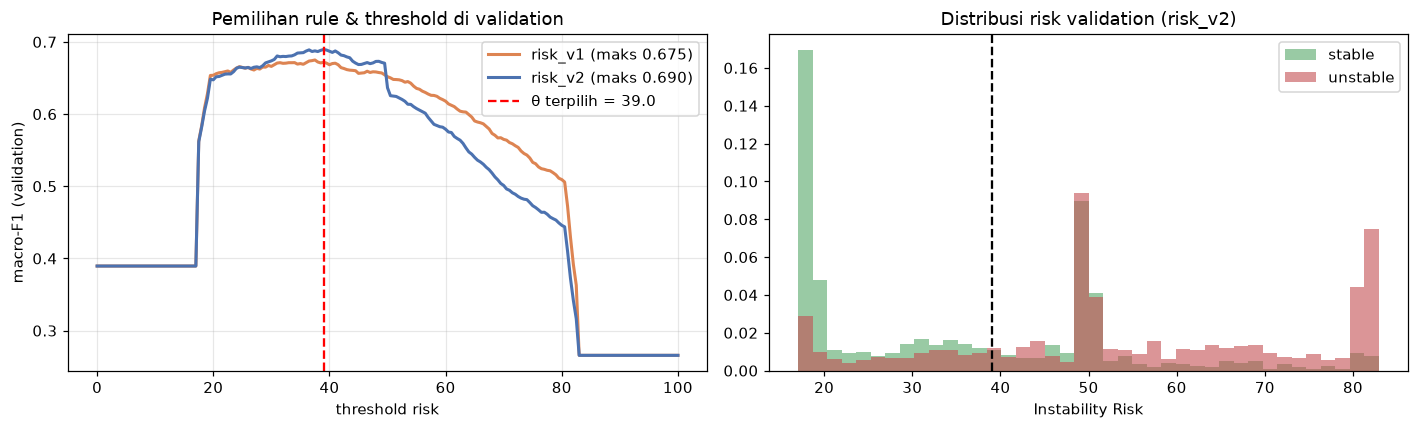
\includegraphics[width=0.62\textwidth]{figures/soal_12_5.png}\hfill
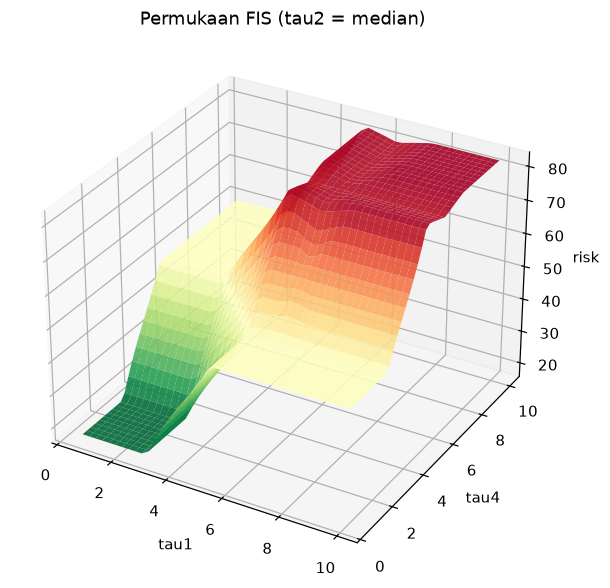
\includegraphics[width=0.36\textwidth]{figures/soal_12_6.png}
\caption{Kiri: pemilihan versi rule dan threshold di validation, serta distribusi risk. Kanan: permukaan FIS ($\tau_2$ = median).}
\end{figure}

\jawab{Jawaban 12d: Perbandingan dengan baseline threshold sederhana}
Baseline-nya satu aturan, ``unstable jika $\tau_1 \geq 3.16$'', dengan batas dipilih dari validation dengan cara yang sama. Logistic regression saya tambahkan sebagai pembanding model statistik.

\begin{adjustbox}{max width=\textwidth}\begin{tabular}{@{}lcccccc@{}}
\toprule
\textbf{Model (test)} & \textbf{Acc} & \textbf{Bal.\ acc} & \textbf{Macro-F1} & \textbf{Recall unst.} & \textbf{Spec.} & \textbf{AUC} \\
\midrule
Baseline $\tau_1 \geq 3.16$ & 0.676 & 0.623 & 0.626 & 0.816 & 0.430 & 0.626 \\
FIS Mamdani v2 & 0.720 & 0.690 & 0.692 & 0.798 & 0.582 & 0.778 \\
Logistic regression & 0.693 & 0.681 & 0.676 & 0.724 & 0.638 & 0.754 \\
\bottomrule
\end{tabular}\end{adjustbox}

Baseline hanya punya satu saklar, sehingga untuk mengejar recall tinggi ia terpaksa menuduh banyak grid stabil sebagai unstable (specificity 0.43). FIS unggul di semua metrik gabungan, dengan macro-F1 lebih tinggi 0.066 dan AUC lebih tinggi 0.15. FIS bahkan sedikit di atas logistic regression, karena rule v2 menangkap efek jenuh yang oleh logistic regression dianggap lurus.

Dari sisi interpretabilitas, setiap keputusan FIS bisa ditelusuri ke rule yang aktif. Sampel dengan $\tau = (9.75, 9.71, 7.65)$, misalnya, mendapat risk 82.9 karena rule ``IF semua High THEN risk High'' aktif 100\%. Rule juga bisa diubah pakar tanpa melatih ulang model. Kekurangannya, skor risk berundak dan sering tepat 17.1, 50, atau 82.9, dan FIS hanya melihat 3 dari 12 fitur sehingga elastisitas $g$ tidak ikut diperhitungkan.

FIS tetap lebih layak walau akurasinya sedikit lebih rendah ketika keputusan harus bisa diaudit, misalnya saat operator harus menjelaskan alasan pelepasan beban. FIS juga cocok ketika data sedikit tetapi ada pengetahuan pakar, ketika yang dibutuhkan peringatan bertingkat (hijau, kuning, merah) dan bukan sekadar ya atau tidak, dan ketika perilaku model harus bisa diperiksa di seluruh ruang input lewat permukaan FIS dan cek celah rule.

\subsection{Interpretasi Hasil}
Dari 20 sampel test, 14 ditebak benar, dengan 4 false alarm dan 2 grid unstable yang terlewat. Tiga dari empat false alarm punya risk sekitar 50, yaitu zona abu-abu yang porsi unstable-nya sekitar 0.67.

\begin{adjustbox}{max width=\textwidth}\begin{tabular}{@{}llll@{}}
\toprule
\textbf{Kriteria} & \textbf{Target} & \textbf{Hasil} & \textbf{Status} \\
\midrule
Rule base lengkap & 0 kosong, 0 aktivasi $< 0.2$ & 0 dan 0 (min 0.50) & \ok{tercapai} \\
FIS $>$ baseline & macro-F1 test & 0.692 vs 0.626 & \ok{tercapai} \\
Ranking skor risk & AUC $\geq 0.70$ & 0.778 & \ok{tercapai} \\
\bottomrule
\end{tabular}\end{adjustbox}

Validasi rule dengan data latih membuktikan bahwa asumsi awal saya keliru: waktu reaksi yang makin lama tidak membuat grid makin berbahaya secara lurus. Rule yang disusun ulang berdasarkan jumlah peserta yang bereaksi cepat lebih akurat dan tetap mudah dibaca. Langkah berikutnya bisa menambah input $g$ lewat hierarchical FIS atau menyetel membership dengan ANFIS.
